\chapter{Realizzazione della modalità "kiosk"}
\label{cha:kiosk}

Nell'ambito dei sistemi \emph{embedded} si utilizza spesso la locuzione \emph{modalità kiosk} per indicare tutte le situazioni in cui il sistema deve comportarsi come un "chiosco digitale" e limitare l'utilizzo a specifiche funzioni. Su Android si possono adottare diverse tecniche per ottenere una modalità simile, nascondendo quindi la presenza del sistema operativo Android. In questo capitolo sono presentate le tecniche sperimentate, tra cui la modalità a schermo intero, la modifica dell'\emph{overscan} di sistema, la modalità \emph{lock task}, l'avvio automatico dell'applicazione e la modifica dell'animazione di avvio del sistema.

\section{La modalità a schermo intero}
\label{sec:kiosk_fullscreen}

A partire da Android 4.1, è stata introdotta una gestione granulare della modalità a schermo intero. Si tratta di base della possibilità di nascondere, utilizzando appositi \emph{flag}, la barra di stato e la barra di navigazione di Android, presenti rispettivamente nella parte superiore e inferiore dello schermo.

\begin{minted}{java}
private void goFullScreen() {
    getWindow().getDecorView().setSystemUiVisibility(
        View.SYSTEM_UI_FLAG_HIDE_NAVIGATION
        | View.SYSTEM_UI_FLAG_FULLSCREEN);
}
\end{minted}

Questo metodo va chiamato sia all'avvio dell'applicazione che nei casi in cui la modalità a schermo intero potrebbe essere automaticamente disabilitata, ovvero quando l'applicazione perde e poi riacquisisce il "focus".

\begin{minted}[highlightlines={4,11}]{java}
@Override
public void onResume(Bundle savedInstanceState) {
    super.onCreate(savedInstanceState);
    goFullScreen();
}

@Override
public void onWindowFocusChanged(boolean hasFocus) {
    super.onWindowFocusChanged(hasFocus);
    if (hasFocus) {
        goFullScreen();
    }
}
\end{minted}


Questa soluzione ha l'effetto di nascondere le due barre di sistema, ma solo fintantoché l'utente non preme un qualsiasi punto dello schermo. Per questo Google ha introdotto anche una "modalità immersiva", che permette di mantenere l'applicazione a schermo intero fino a quando l'utente non scorre dai bordi dello schermo, come mostrato in seguito.\footnote{\url{https://developer.android.com/training/system-ui/immersive}}

\begin{figure}
\begin{minted}[highlightlines={7,9,10,11}]{java}
private void goFullScreen() {
    getWindow().getDecorView().setSystemUiVisibility(
        // Nasconde barra di navigazione e di stato
        View.SYSTEM_UI_FLAG_HIDE_NAVIGATION
        | View.SYSTEM_UI_FLAG_FULLSCREEN
        // Modalità immersiva
        View.SYSTEM_UI_FLAG_IMMERSIVE_STICKY
        // Evita lo spostamento del layout della pagina
        | View.SYSTEM_UI_FLAG_LAYOUT_STABLE
        | View.SYSTEM_UI_FLAG_LAYOUT_HIDE_NAVIGATION
        | View.SYSTEM_UI_FLAG_LAYOUT_FULLSCREEN);
}
\end{minted}
\end{figure}


\section{L'\emph{overscan} di sistema}
\label{sec:kiosk_overscan}

Come accennato, la modalità a schermo intero di Android permette comunque all'utente di usare le barre di sistema scorrendo dai lati dello schermo, e quindi potenzialmente di uscire dall'applicazione. In un sistema embedded questo non è desiderabile, ed esiste quindi un metodo alternativo per impedire che le barre di sistema vengano mostrate.

La soluzione prevede l'utilizzo della funzione \emph{overscan} del servizio di sistema \texttt{WindowManager}, il quale si occupa di gestire la visualizzazione delle finestre, la rotazione dello schermo, le animazioni, le transizioni, ecc.

L'overscan di sistema permette di modificare l'area di disegno delle finestre, o in altre parole i margini dello schermo. Impostando un margine negativo l'area di disegno dell'interfaccia di Android sarà estesa oltre l'area visibile dello schermo, con l'effetto di tagliare porzioni dell'interfaccia, come mostrato nella figura \ref{fig:overscan}.

\begin{figure}[h]
	\centering
	
	\scalebox{0.5} {
		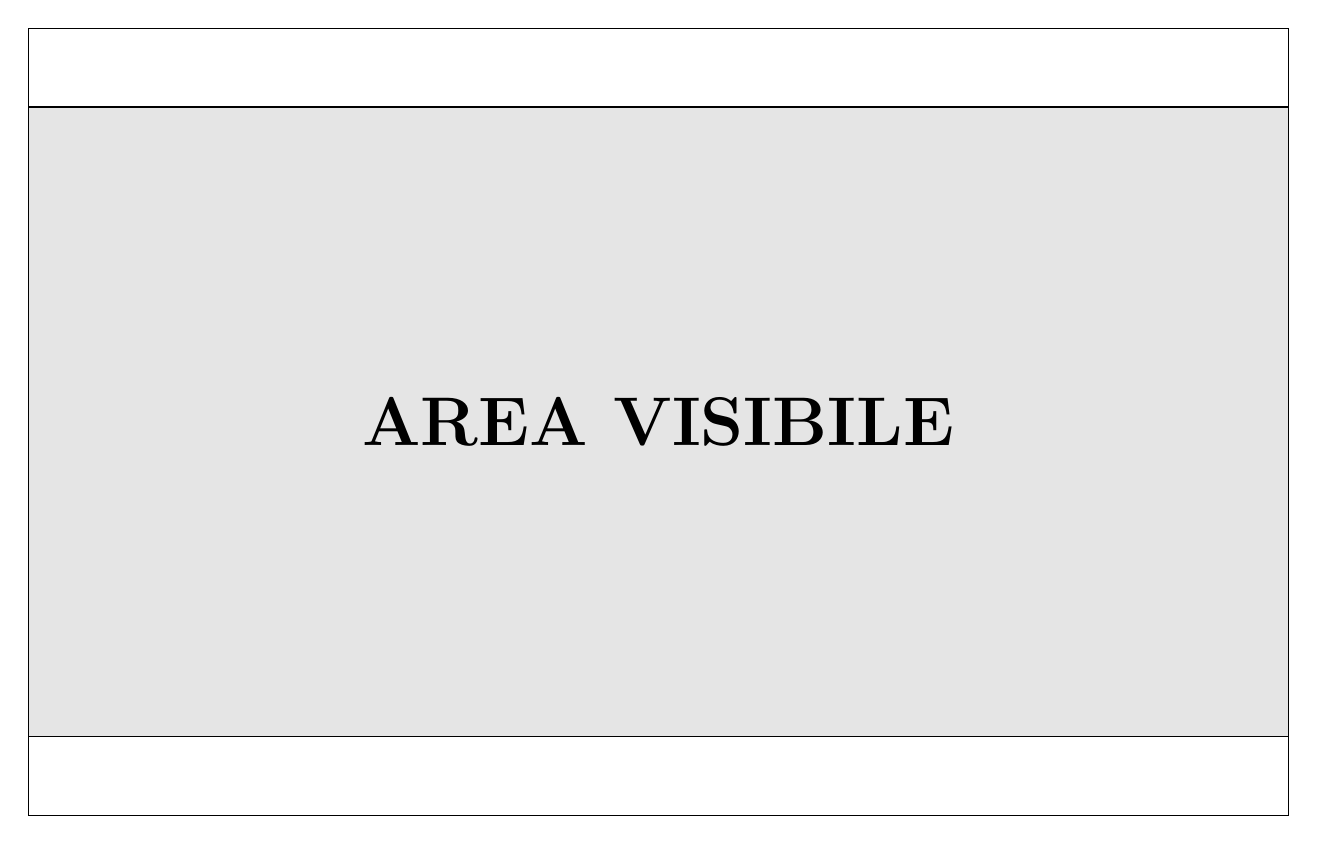
\begin{tikzpicture}
		\filldraw[fill=white,draw=black]
		(0,0) rectangle (16,10);
		\filldraw[fill=black!10,draw=black]
		(0,1) rectangle (16,9) node[midway,text=black] {\Huge \textbf{AREA VISIBILE}};
		\end{tikzpicture}
	}

	\caption{Rappresentazione dell'overscan di sistema. La finestra sconfina l'area visibile.}
	\label{fig:overscan}
\end{figure}

Nell'esempio seguente viene utilizzato il comando \texttt{wm} (\texttt{WindowManager}) della shell di Android per impostare un margine negativo al lato superiore e inferiore dello schermo, in modo da nascondere barra di stato e di navigazione, alte in questo caso 25dp e 48dp\footnote{Density-independent Pixels, un'unità di misura che tiene in considerazione la densità dello schermo} (i valori possono essere diversi a seconda del dispositivo).

\begin{minted}[highlightlines=9]{bash}
> adb shell wm
usage: wm [subcommand] [options]
wm size [reset|WxH|WdpxHdp]
wm density [reset|DENSITY]
wm overscan [reset|LEFT,TOP,RIGHT,BOTTOM]

> adb shell wm overscan 0,-25,0,-48
\end{minted}

Una volta configurato l'overscan, l'impostazione dovrebbe essere memorizzata in modo permanente e sopravvivere al riavvio del sistema. Tuttavia, durante le sperimentazioni si è verificato almeno una volta che l'overscan non fosse ripristinato in automatico. Potrebbe quindi essere opportuno eseguire il comando ad ogni avvio del sistema, anche avviando un processo dall'applicazione stessa.

Per completezza, l'overscan può essere disabilitato con questo comando:

\begin{minted}{bash}
> adb shell wm overscan reset
\end{minted}


\section{La modalità "lock task"}
\label{sec:kiosk_locktask}

In aggiunta ai metodi illustrati nei capitoli precedenti, Android fornisce a partire dalla versione 5.0 una modalità chiamata \emph{lock task}, che fa parte di un insieme più ampio di API per la realizzazione di dispositivi dedicati (in passato chiamati COSU, Corporate-Owned Single-Use). Queste API fanno a loro volta parte di Android Enterprise, che propone soluzioni specifiche per casi d'uso aziendali.

Quando la modalità lock task viene abilitata, il sistema operativo entra in una modalità rigida che permette di usare solo un insieme di applicazioni definite manualmente tramite una \emph{whitelist}. Inoltre, la barra di stato viene disabilitata, le notifiche sono soppresse, e l'utilizzatore non può navigare nel sistema al di fuori delle app inserite in whitelist.\footnote{\url{https://developer.android.com/work/dpc/dedicated-devices/lock-task-mode}}

\begin{figure}[h]
	\centering
	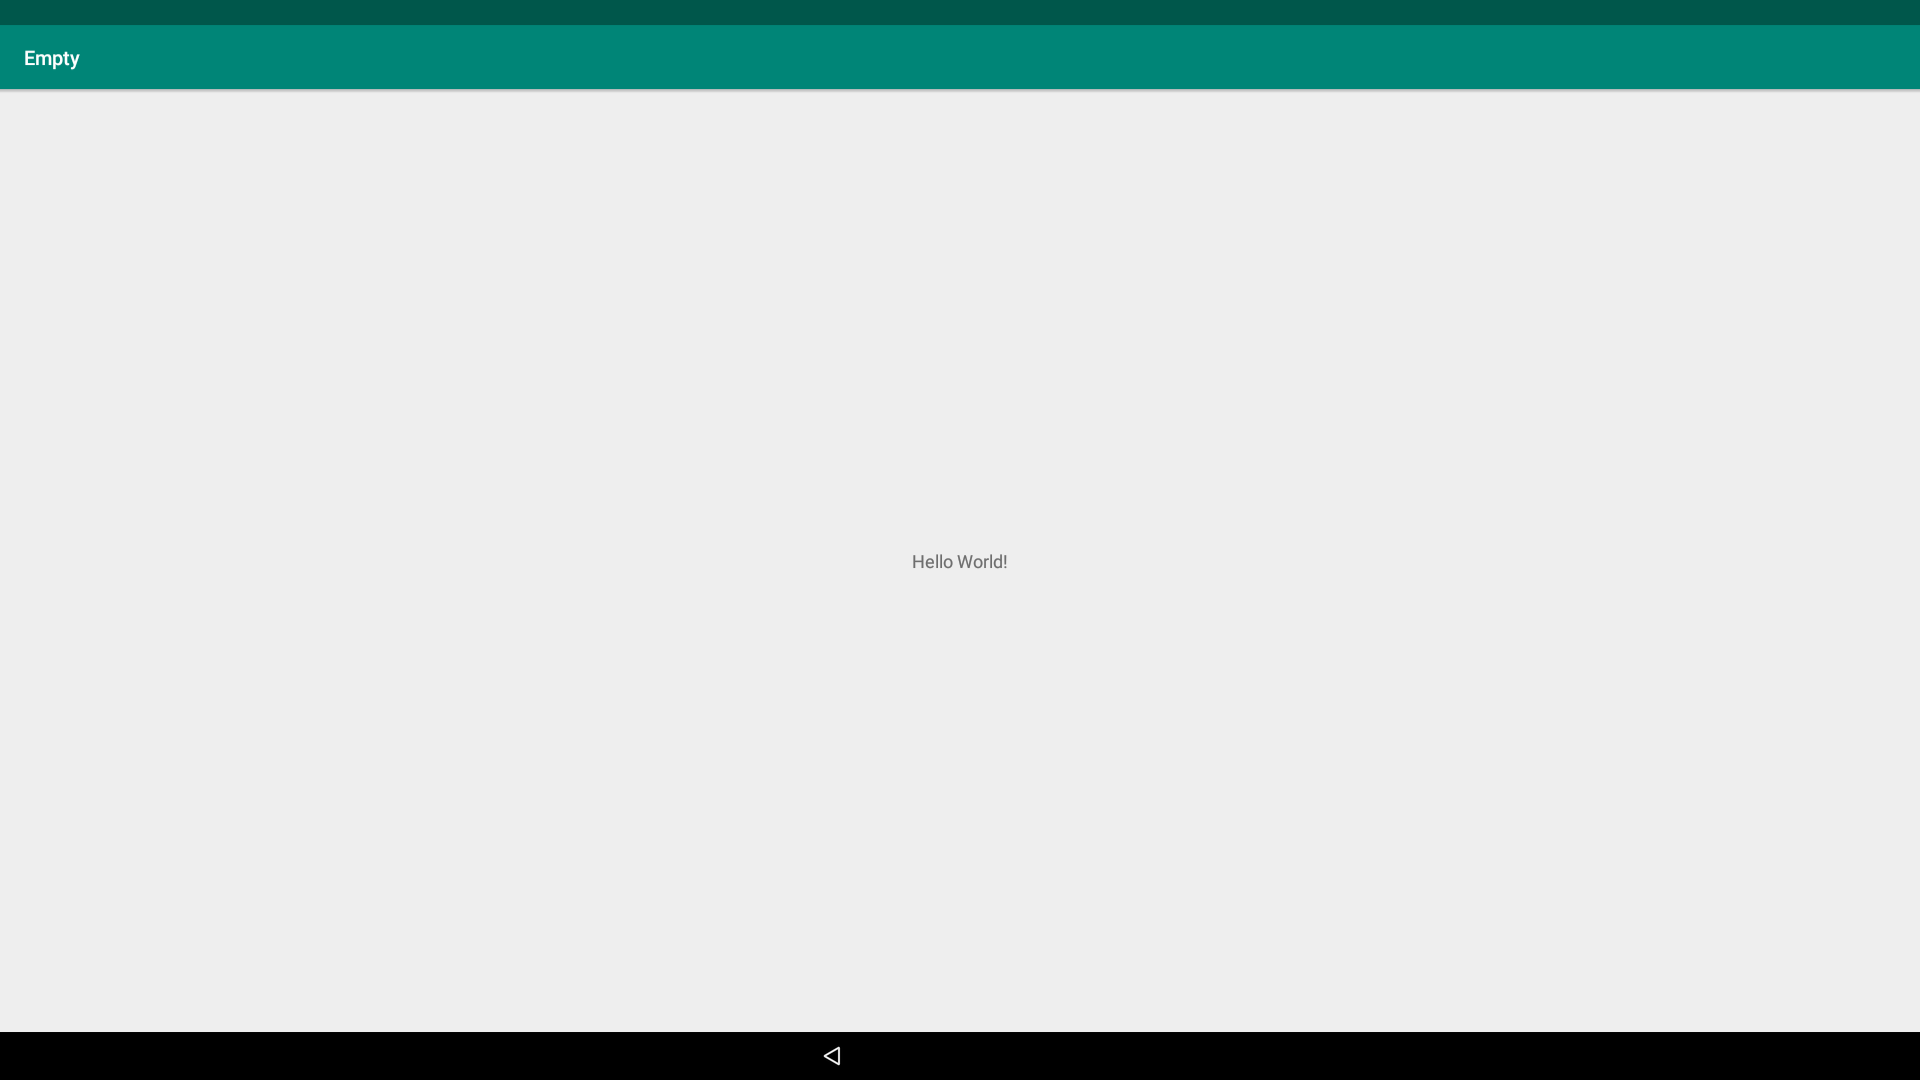
\includegraphics[width=0.8\textwidth]{res/locktask.png}
	
	\caption{In modalità lock task la barra di stato e di navigazione sono disabilitate.}
	\label{fig:kiosk_locktask}
\end{figure}

Per implementare la modalità lock task sono necessari due componenti: un Device Policy Controller (DPC) e una \texttt{Activity} da lanciare. Il DPC deve essere un'applicazione "proprietaria del dispositivo", e cioè deve avere dei privilegi speciali per modificare alcune funzioni di sistema. Ha infatti il compito di configurare la modalità lock task elencando i nomi dei \emph{package} da inserire in whitelist.

La procedura per la realizzazione di un DPC è articolata ed è dettagliata nella documentazione di Android\footnote{\url{https://developer.android.com/guide/topics/admin/device-admin.html\#developing}}, ma è sufficiente sapere che viene fornito un metodo per scegliere quali applicazioni possono essere eseguite in modalità lock task:

\begin{minted}[highlightlines=4]{java}
DevicePolicyManager dpm =
    (DevicePolicyManager) getSystemService(Context.DEVICE_POLICY_SERVICE);
ComponentName adminName = getComponentName(this);
dpm.setLockTaskPackages(adminName, new String[] { "it.unitn.lode" });
\end{minted}

Google fornisce inoltre un'applicazione chiamata "Test DPC" che implementa numerose funzionalità legate alle policy aziendali, tra cui la configurazione della whitelist. L'applicazione è particolarmente utile durante lo sviluppo, perché permette di effettuare test rapidamente senza sviluppare un DPC. L'installazione è semplice e prevede di impostare "Test DPC" come proprietario del dispositivo:\footnote{\url{https://codelabs.developers.google.com/codelabs/cosu/index.html\#6}}

\begin{minted}{bash}
> adb install TestDPC.apk
> adb shell dpm set-device-owner com.afwsamples.testdpc/.DeviceAdminReceiver
\end{minted}

A questo punto, la \texttt{Activity} che vuole entrare in modalità lock task può semplicemente chiamare il metodo \texttt{startLockTask()}:

\begin{minted}[highlightlines=9]{java}
@Override
public void onResume() {
    super.onResume();
    
    DevicePolicyManager dpm =
        (DevicePolicyManager) getSystemService(Context.DEVICE_POLICY_SERVICE);

    if (dpm.isLockTaskPermitted(getPackageName())) {
        startLockTask();
    }
}
\end{minted}

Se ben configurata, questa soluzione, combinata con le tecniche mostrate nei capitoli precedenti, permette di avere un'applicazione a schermo intero da cui è impossibile uscire.

\section{L'avvio automatico dell'applicazione}
\label{sec:kiosk_launcher}

Una \texttt{Activity} può essere configurata per sostituire la schermata "home" di Android, ed essere quindi la prima ad essere mostrata all'avvio del sistema.

Il blocco di codice seguente mostra una porzione del file \texttt{AndroidManifest.xml}, tramite il quale è stato forzato il fatto che possa esistere una sola istanza alla volta di \texttt{MainActivity}, e che questa debba agire come attività "home" predefinita:

\begin{minted}[highlightlines={2,6,7}]{xml}
<activity android:name=".MainActivity"
          android:launchMode="singleTask">
    <intent-filter>
        <action android:name="android.intent.action.MAIN"/>
        <category android:name="android.intent.category.LAUNCHER"/>
        <category android:name="android.intent.category.DEFAULT" />
        <category android:name="android.intent.category.HOME" />
    </intent-filter>
</activity>
\end{minted}

\section{L'animazione di avvio}
\label{sec:kiosk_bootanimation}

Come ultimo aspetto, un requisito di un sistema embedded potrebbe essere quello di non mostrare i marchi di Android o del produttore dell'hardware. Fortunatamente, Android permette in modo abbastanza facile di sostituire l'animazione di avvio del sistema con una a piacere.\footnote{\url{https://android.googlesource.com/platform/frameworks/base/+/master/cmds/bootanimation/FORMAT.md}}

In fase di avvio, il sistema legge il file \texttt{/system/media/bootanimation.zip} ed estrae una descrizione dell'animazione (\texttt{desc.txt}) e un insieme di file PNG rappresentanti i fotogrammi da mostrare in sequenza su schermo.

Per fare un esempio, si prenda come riferimento questo file di descrizione:

\begin{minted}{text}
400 200 10
c 0 0 part0 #ffffff
\end{minted}

La prima riga indica parametri generali dell'animazione, in particolare la larghezza, l'altezza e il numero di fotogrammi al secondo da renderizzare.

La seconda riga indica invece un blocco di fotogrammi che devono essere eseguiti secondo precise regole. In particolare:

\begin{itemize}
	\item la lettera \texttt{c} indica che l'animazione verrà eseguita fino al suo completamento, anche nel caso in cui il sistema sia pronto prima;
	\item la prima occorrenza del numero \texttt{0} indica quante volte l'animazione deve essere ripetuta, in questo caso infinite volte, mentre la seconda il numero di fotogrammi di attesa prima della riproduzione del blocco successivo;
	\item \texttt{part0} è il nome della cartella in cui trovare la lista di file che compongono l'animazione;
	\item infine, l'ultimo parametro determina il colore di sfondo nel caso in cui l'animazione sia trasparente o non copra l'intero schermo.
\end{itemize}

I file ottenuti possono quindi essere inseriti in un archivio ZIP senza compressione, con un comando simile a questo:

\begin{minted}{bash}
zip -0qry -i \*.txt \*.png @ ../bootanimation.zip *.txt part*
\end{minted}

Infine, il file \texttt{bootanimation.zip} va caricato sul dispositivo Android tramite \texttt{adb} e la modalità debug con accesso root:

\begin{minted}{bash}
adb root
adb remount
adb push bootanimation.zip /system/media
adb reboot
\end{minted}

